\subsection{Descriptive Data Analysis}
\label{sec:dda}

Developing machine learning models for predicting certain outcomes requires
an understanding of the underlying data.
Insights derived from descriptive data analysis are useful in all steps of the
modeling process, e.g., for preprocessing, feature extraction and evaluation
of model performance.
For this thesis, exploratory data analysis also serves the purpose of establishing
differences between the three examined data sets.
The upcoming sections compare the collected data sets along the dimensions of
engagement metrics (ch.~\ref{sec:engagement_stats}), network characteristics
(ch.~\ref{sec:network_stats}) and general account activity (ch.~\ref{sec:activity_stats}).
Prior to presenting the results of this analysis, a few remarks about presentation
have to be made.
In almost all cases, data is discretized to improve clarity.
Here, all created bins, e.g., in histograms, are left-inclusive and right-exclusive.
For example, the bin `1-10k' denotes all observations between 1,000 and
9,999 (for a variable scaled as an integer).
In addition, all represented distributions are normalized to account for varying
data set sizes and improve comparability.
Diagrams for the combined data set are omitted at times, mainly when the observed
distibution closely resembles the other data sets.

\subsubsection{Engagement statistics}
\label{sec:engagement_stats}

Examining engagement statistics for all three data sets is crucial since the goal
of this thesis is to predict these variables.
This section will therefore compare retweet and favorite distribution for 
celebrity, politician and corporate tweets.

\begin{table}[h]
\begin{tabular}{lrrrr}
\toprule
  Retweets & Celebrities & Politicians & Companies & Combined\\
\midrule
  Mean & 1,629.8 & 318.4 & 15.1 & 286.2\\
  Median & 176.0 & 23.0 & 1.0 & 3.0 \\
\midrule
  Favorites & Celebrities & Politicians & Companies & Combined\\
\midrule
  Mean & 6,135.6 & 832.9 & 40.3 & 908.8 \\
  Median & 1117.0 & 69.0 & 1.0 & 5.0 \\
\midrule
  Pearson correlation & Celebrities & Politicians & Companies & Combined\\
\midrule
  Correlation coefficient & 0.9188 & 0.9457 & 0.9803 & 0.9132\\
\bottomrule
\end{tabular}
\caption{Summary of engagement statistics}
\label{tab:engagement_summary}
\end{table}

Table~\ref{tab:engagement_summary} indicates that celebrity tweets are engaged
with most often.
This holds true when looking at central tendency statistics (mean and median)
for retweet and favorite counts.
Moreover, in this sample politician tweets are more popular compared to tweets from corporate
accounts.
For all data sets, strong correlation between the number of favorites and retweets can
be stated.
This observation is useful for later model development, because it can be concluded that
both variables should be predictable using similar statistical models, e.g.,
a multi-output model with differently scaled weights in the last layer.
The differences between mean and median values point to skewness in the
underlying distributions.
Since the calculated means are significantly larger than their respective
median values, observations should extend farther to the right
of the distributions.
This finding can be explained twofold. 
Firstly, retweet and favorite counts have an obvious  minimum of zero.
Secondly, a small number of very popular tweets constitute outliers which largely
influence the mean calculation.
In order to examine engagement distributions in more detail, Fig.~\ref{fig:retw_distr} and
Fig.~\ref{fig:fav_distr} illustrate engagement statistics which are discretized into logarithmic bins (base 10).
Above discretization also corresponds to the classes used for the classification models
of this thesis.

\begin{figure}[h]
\begin{subfigure}{.45\textwidth}
  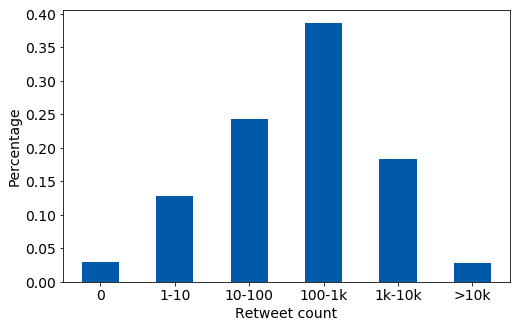
\includegraphics[width=.95\linewidth]{img/celeb_retw_distr}
  \caption{Celebrity data set}
  \label{fig:retw_distr_sub1}
\end{subfigure}%
\begin{subfigure}{.45\textwidth}
  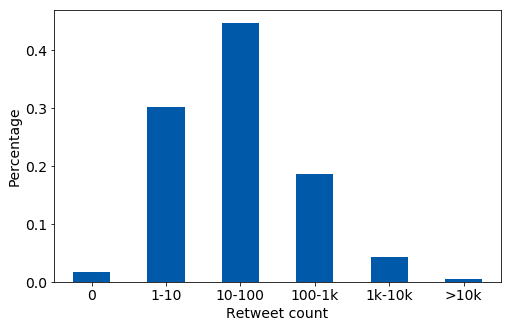
\includegraphics[width=.95\linewidth]{img/polit_retw_distr}
  \caption{Politician data set}
  \label{fig:retw_distr_sub2}
\end{subfigure}
\begin{subfigure}{.45\textwidth}
  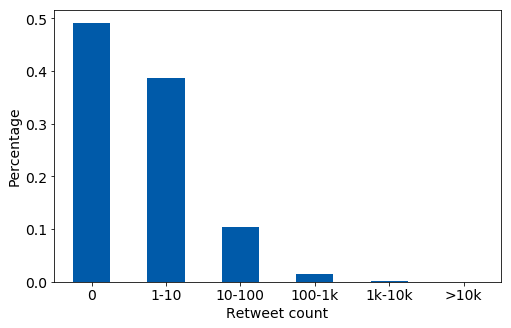
\includegraphics[width=.95\linewidth]{img/corp_retw_distr}
  \caption{Company data set}
  \label{fig:retw_distr_sub3}
\end{subfigure}%
\begin{subfigure}{.45\textwidth}
  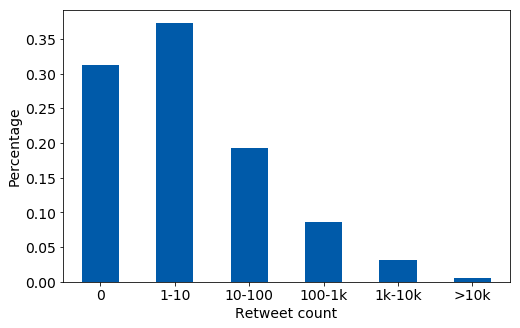
\includegraphics[width=.95\linewidth]{img/comb_retw_distr}
  \caption{Combined data set}
  \label{fig:retw_distr_sub4}
\end{subfigure}%
\caption{Retweet distributions}
\label{fig:retw_distr}
\end{figure}

\begin{figure}[h]
\begin{subfigure}{.45\textwidth}
  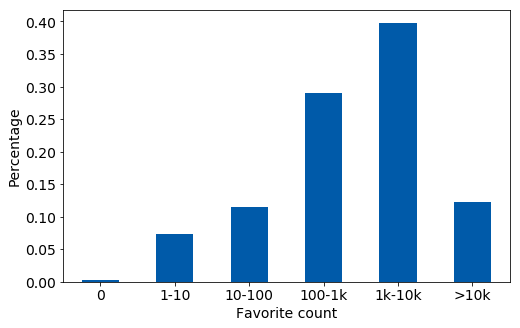
\includegraphics[width=.95\linewidth]{img/celeb_fav_distr}
  \caption{Celebrity data set}
  \label{fig:fav_distr_sub1}
\end{subfigure}%
\begin{subfigure}{.45\textwidth}
  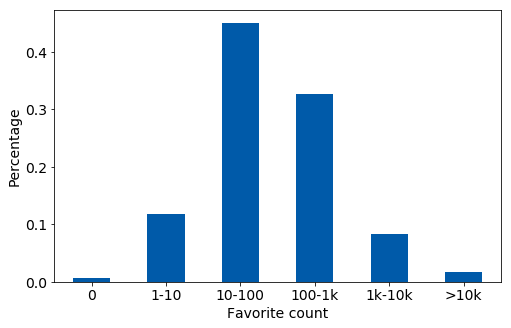
\includegraphics[width=.95\linewidth]{img/polit_fav_distr}
  \caption{Politician data set}
  \label{fig:fav_distr_sub2}
\end{subfigure}
\begin{subfigure}{.45\textwidth}
  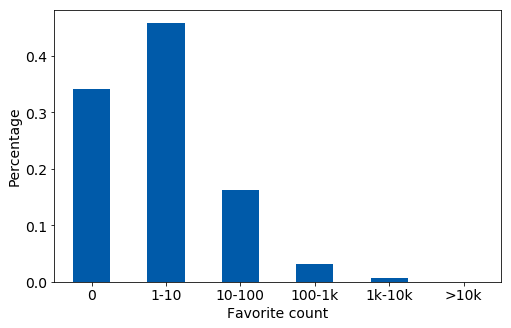
\includegraphics[width=.95\linewidth]{img/corp_fav_distr}
  \caption{Company data set}
  \label{fig:fav_distr_sub3}
\end{subfigure}%
\begin{subfigure}{.45\textwidth}
  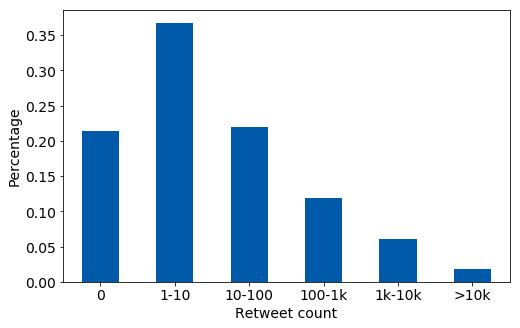
\includegraphics[width=.95\linewidth]{img/comb_fav_distr}
  \caption{Combined data set}
  \label{fig:fav_distr_sub4}
\end{subfigure}%
\caption{Favorite distributions}
\label{fig:fav_distr}
\end{figure}

All three data sets possess class imbalance, i.e., some classes are more likely
to occur than others.
Here, differences in class probabilities are significant across data sets
and variables, with the most common class
containing close to or more than 40\% of all observations and some classes
hardly being represented at all.
Looking at retweets it can be stated that celebrity and politician distributions
have a Gaussian-like shape, where the central tendency of celebrity tweets is
farther to the right.
Company retweet classes seem to be more exponentially shaped.
Moving to favorites, central tendencies of all distributions are clearly pushed to the right of the
spectrum, which accounts for the generally observed difference between favorite
and retweet counts.
As can be expected, class distributions in the combined data set resemble a
weighted average of the other data sets.
As a consequence, class imbalance is less extreme for this data set.

The upcoming subsections further describe characteristics of the collected
data sets and provide possible explanations of the found discrepancies in
retweet and favorite distributions.

\subsubsection{Network statistics}
\label{sec:network_stats}

Prior work in this area suggests the importance of user data when predicting
popularity of created tweets.
The most obvious features in this category are the number of incoming and outgoing
connections, i.e., follower and friend counts in the context of Twitter.
This section shows the distribution of these variables in the previously
defined user groups and examines the correlation with engagement metrics.

\begin{table}
\begin{tabular}{lrrrr}
\toprule
  Number of followers & Celebrities & Politicians & Companies & Combined\\
\midrule
  Mean & 10,255,423 & 331,944 & 357,023 & 2,170,010\\
  Median & 3,228,642 & 89,072 & 23,204 & 92,273\\
  Correlation w/ retweets & 0.1457 & 0.2828 & 0.0326 & 0.2947\\
  Correlation w/ favorites & 0.1922 & 0.3423 & 0.0442 & 0.3396\\
\midrule
  Number of friends & Celebrities & Politicians & Companies & Combined\\
\midrule
  Mean & 5,587 & 3,775 & 5,513 & 4,942\\
  Median & 241 & 599 & 800 & 1,055\\
  Correlation w/ retweets & 0.1799 & 0.0030 & -0.0036 & 0.1967\\
  Correlation w/ favorites & 0.1754 & 0.0092 & -0.0049 & 0.1617\\
\bottomrule
\end{tabular}
\caption{Summary of network statistics}
\label{tab:network_summary}
\end{table}

\begin{figure}[h]
\begin{subfigure}{.33\textwidth}
  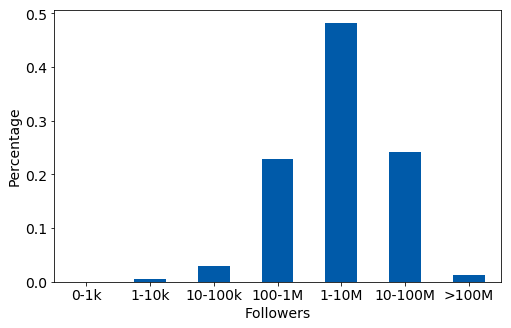
\includegraphics[width=.95\linewidth]{img/celeb_follow_distr}
  \caption{Celebrity data set}
  \label{fig:follow_distr_sub1}
\end{subfigure}%
\begin{subfigure}{.33\textwidth}
  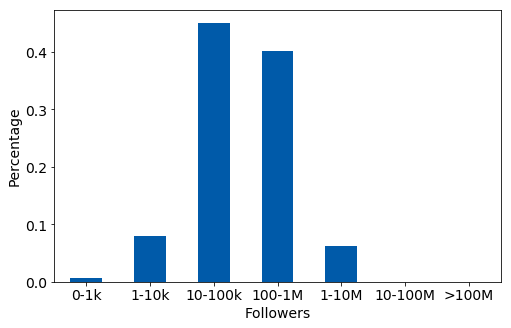
\includegraphics[width=.95\linewidth]{img/polit_follow_distr}
  \caption{Politician data set}
  \label{fig:follow_distr_sub2}
\end{subfigure}
\begin{subfigure}{.33\textwidth}
  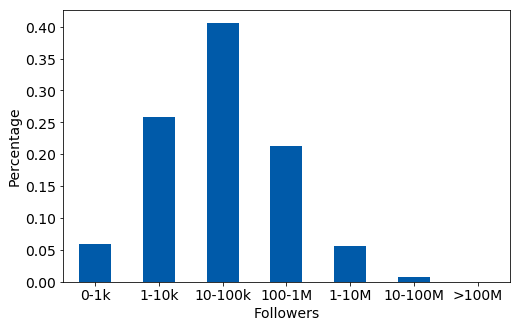
\includegraphics[width=.95\linewidth]{img/corp_follow_distr}
  \caption{Company data set}
  \label{fig:follow_distr_sub3}
\end{subfigure}%
\caption{Follower distributions}
\label{fig:follow_distr}
\end{figure}

Table~\ref{tab:network_summary} summarizes network statistics for all three
user groups.
It can be stated that celebrities tend to have the largest following on average,
followed by companies and politicians.
Most celebrities are followed by more than a million accounts, whereas the
majority of politicans and companies have followings smaller than 100 thousand
accounts (see Fig.~\ref{fig:follow_distr}).
Again, follower and friend distributions are skewed to the right across all
groups.
Considering the previously demonstrated differences in retweet and favorite
distributions, one could assume a correlation between number of followers
and tweet popularity.
However, linear correlation with retweet and favorites counts is nonexistent
(celebrities and companies) or only weakly positive (politicians).
Correlation coefficients are even lower for the number of friends a user
possesses.
The friend distributions have a similar shape, more than half of all users
follow less than 1,000 accounts (see Fig.~\ref{fig:friend_distr}).
The median value is highest for corporate accounts which seems logical, since
these accounts are probably most often managed using more manpower.
Particularly strong linear relationships between number of friends and engagement statistics can not
be found.
Correlation coefficients are higher for the combined data set, but still not
significant.
Since the majority of users come from the company user group, follower and friend
distributions for the combined data set are very similar to the ones of this group.
Illustration is thus omitted for the sake of brevity.

\begin{figure}[h]
\begin{subfigure}{.33\textwidth}
  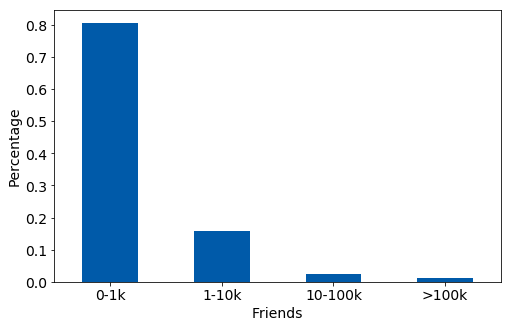
\includegraphics[width=.95\linewidth]{img/celeb_friend_distr}
  \caption{Celebrity data set}
  \label{fig:friend_distr_sub1}
\end{subfigure}%
\begin{subfigure}{.33\textwidth}
  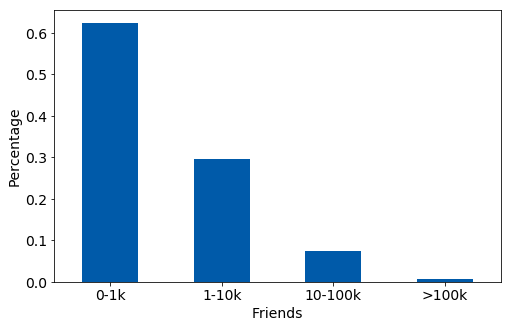
\includegraphics[width=.95\linewidth]{img/polit_friend_distr}
  \caption{Politician data set}
  \label{fig:friend_distr_sub2}
\end{subfigure}
\begin{subfigure}{.33\textwidth}
  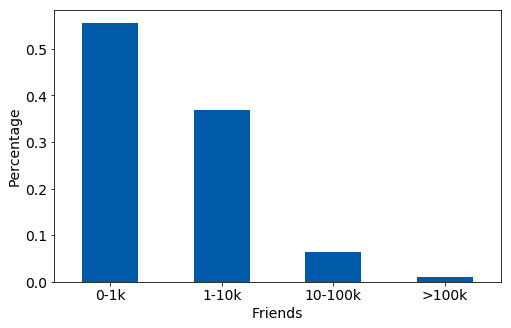
\includegraphics[width=.95\linewidth]{img/corp_friend_distr}
  \caption{Company data set}
  \label{fig:friend_distr_sub3}
\end{subfigure}%
\caption{Friend distributions}
\label{fig:friend_distr}
\end{figure}

\subsubsection{Activity statistics}
\label{sec:activity_stats}

Like network data, activity statistics have been used as features in previously
developed models which serve the purpose of retweet prediction.
Both feature groups can be classified in the category of contextual features,
as opposed to content features.
This section will describe account age and tweet frequency as indicators
for user activity.

\begin{figure}[h]
\begin{subfigure}{.33\textwidth}
  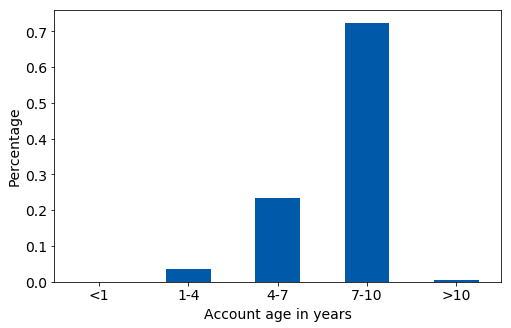
\includegraphics[width=.95\linewidth]{img/celeb_age_distr}
  \caption{Celebrity data set}
  \label{fig:age_distr_sub1}
\end{subfigure}%
\begin{subfigure}{.33\textwidth}
  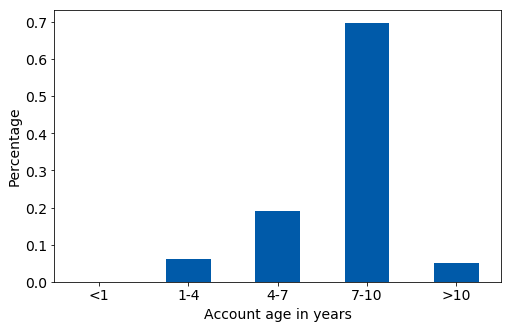
\includegraphics[width=.95\linewidth]{img/polit_age_distr}
  \caption{Politician data set}
  \label{fig:age_distr_sub2}
\end{subfigure}
\begin{subfigure}{.33\textwidth}
  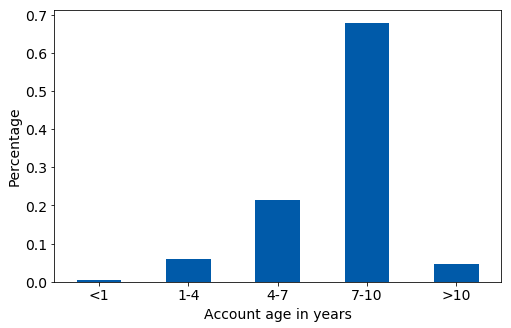
\includegraphics[width=.95\linewidth]{img/corp_age_distr}
  \caption{Company data set}
  \label{fig:age_distr_sub3}
\end{subfigure}%
\caption{Account age distributions}
\label{fig:age_distr}
\end{figure}

Fig.~\ref{fig:age_distr} shows the account age distributions, calculated for
each user group individually.
Superficially, the distributions look similar.
For all groups, around 70\% of all accounts are seven to ten years old, thus being
created two to four years after Twitter was opened for public access.
Earlier adopters mainly stems from the politician and company user groups, about
5\% of accounts in these groups are older than ten years.
There is hardly any skewness in the account age distribution, i.e., median and
mean values are close to each other.

\begin{figure}[h]
\begin{subfigure}{.33\textwidth}
  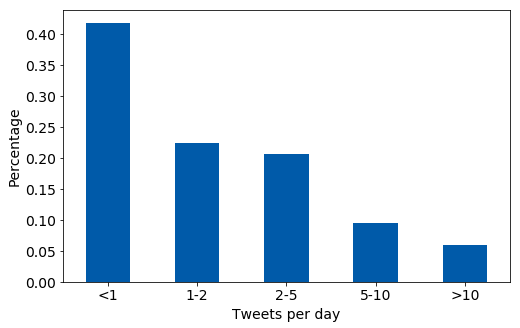
\includegraphics[width=.95\linewidth]{img/celeb_freq_distr}
  \caption{Celebrity data set}
  \label{fig:freq_distr_sub1}
\end{subfigure}%
\begin{subfigure}{.33\textwidth}
  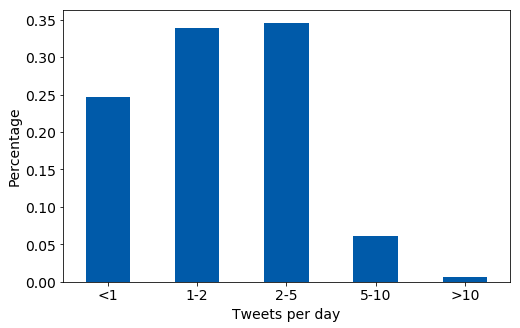
\includegraphics[width=.95\linewidth]{img/polit_freq_distr}
  \caption{Politician data set}
  \label{fig:freq_distr_sub2}
\end{subfigure}
\begin{subfigure}{.33\textwidth}
  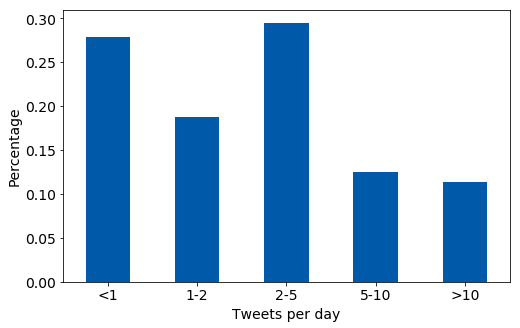
\includegraphics[width=.95\linewidth]{img/corp_freq_distr}
  \caption{Company data set}
  \label{fig:freq_distr_sub3}
\end{subfigure}%
\caption{Tweet frequency distributions}
\label{fig:freq_distr}
\end{figure}

Although accounts exemplify rougly the same age distribution across all user
groups, their activity level differ considerably (see Fig.~\ref{fig:freq_distr}).
Many celebrities do not average one tweet per day and the median for this group (1.20)
is lower than the respective counterparts for politicians and companies (1.75 resp. 2.16).
However, these numbers are not surprising, since many companies employ Twitter accounts
for daily customer support.
This could also explain the high percentage of accounts with more than ten tweets
per day in this group (so-called \textit{power users}).
It can also be stated that users from the politician user group tend to concentrate
in the range of under five tweets per day.
The 75th percentile is the lowest for all three user groups (2.83 tweets per day).
Neither account age nor tweet frequency show any direct linear correlation with
retweet or favorite counts for the collected tweets.
In more detail, all correlation coefficients are located between -0.1 and 0.1 (all
calculated values can be found in the appendix of this thesis).

This section concludes the descriptive data analysis part of this thesis.
Observations derived from these analyses are used in subsequent sections,
particularly for feature extraction and performance evaluation.
